\documentclass{article}

\usepackage{ragged2e}
\usepackage{booktabs}
\usepackage{multirow}
\usepackage{graphicx}
\usepackage{amsmath}
\usepackage[style=alphabetic]{biblatex}
    \addbibresource{main.bib}

\newcommand{\mup}{$\mu$P}
\newcommand{\mutransfer}{$\mu$Transfer}
\newcommand{\fanin}{\text{fan-in}}
\newcommand{\fanout}{\text{fan-out}}
\newcommand{\cinput}{c_{\text{input}}}
\newcommand{\chidden}{c_{\text{hidden}}}
\newcommand{\coutput}{c_{\text{output}}}
\newcommand{\kinput}{k_{\text{input}}}
\newcommand{\khidden}{k_{\text{hidden}}}
\newcommand{\koutput}{k_{\text{output}}}

\title{Does Maximal Feature Learning yield better features?}
\author{
Georgios Vlassis\\
gvlassis@ethz.ch
\and
Lorenzo Noci\\
lorenzo.noci@ethz.ch
}
\date{\today}

\begin{document}

\maketitle

\section{Abstract}
In the field of Deep Neural Networks, a \textit{parametrization} is defined as a prescription according to which the weights of a network are initialized and updated. In the Tensor Programs (TP) framework, the Maximal Update Parametrization (\mup) has been proposed as the parametrization that maximizes "feature" learning in the infinite-width limit. Here, ``feature'' refers to the intermediate activations of the network, which, at an intuitive level, correspond to the ``concepts'' the network learns in order to solve the upstream task. \mup\ is maximal at infinite-width in the sense that any other parametrization has a trivial limit there. Hence, \mup\ should be expected to learn more meaningful representations. Even though this was the original motivation of \mup, subsequent works have mainly focused on its upstream performance. In this work, we instead investigate if the features learned by \mup\ are indeed better than those learned by the Standard Parametrization (SP). We chose Language Modeling (LM) pretraining as our upstream task, and perform a quantitative and qualitative comparison of the two parametrizations. Our results suggest that \mup\ can indeed lead to better features, although indirectly, by enabling the network to achieve better upstream performance.

\section{Introduction}
\subsection{Related works}
Perhaps the most alluring property of DNN is their ability to automatically learn strong representations. This has allowed Deep Learning researchers to sidestep the laborious handcrafting of features, while simultaneously achieving state of the art performance in nearly every Computer Vision and Natural Language Processing task. This trend, started by AlexNet \cite{alexnet} in 2012, has been succeeded by another trend: the self-supervised pretraining of big models with massive amounts of unlabeled data, followed by supervised training on small datasets. During the first stage, the models acquire general representations that would not be able to learn just by training on the small datasets, which significantly improve downstream performance. Probably the most well known models that employ this are the Generative Pretrained Transformer (GPT) \cite{gpt1,gpt2,gpt3,gpt4} and the Bidirectional Encoder Representation Transformer (BERT) \cite{bert}.

Here with the word ``features'' we refer to the outputs of the activation function of intermediate layers of a network. Even though most currently used initialization schemes ensure that activations are initially $\mathcal{O}(1)$ with respect to the width of the network, this condition is violated during training, possibly causing wide networks to diverge \cite{tp4}. In fact, \cite{tp4,tp5}, using theory from the TP series of papers \cite{tp0,tp1,tp2,tp2b,tp3,tp4,tp4b,tp4c,tp5,tp6}, proposed the \mup\ parametrization, which is claimed to be the \textit{unique} parametrization that leads to a non-trivial limit at infinite-width. Although \mup\ has additional advantages over SP, most importantly enabling hyperparameter transfer from narrow to wide networks (\mutransfer) \cite{tp5}, the original motivation behind it was the stabilization of features with respect to width, with the implied expectation that it would lead to better features.

Indeed, subsequent works mostly focus on \mutransfer, either trying to theoretically explain it \cite{noci}, or utilizing it to achieve better upstream performance \cite{cerebras} (Cerebras-GPT), \cite{flm} (FLM-101B), \cite{btlm} (BTLM-3B-8K), \cite{cc} (CrystalCoder), \cite{minicpm} (MiniCPM), \cite{teleflm} (Tele-FLM) and \cite{graphium} (Graphium).

\subsection{Methods}
In contrast to these works, we study the effect of \mup on features. We focus on the Language Modeling (LM) objective using transformer models (based on the GPT2 architecture). As our pretraining dataset, we employ Open WebText \cite{owt}. We trained networks of widths $\zeta \times 64$ for $\zeta \in \{1,2,4,8,16\}$, under both SP and \mup. Our biggest models coincide with GPT2-small (117M parameters), and indeed atain similar upstream performance after being trained for 100B tokens.

After pretraining, we finetune on top of the features learned during LM on five tasks and nine datasets. We then plot downstream performance versus the width multiplier $\zeta$ for both SP and \mup. Our goal is to compare the two parametrizations quantitatively as the width is scaled. We moreover directly compare the distribution of features at inference as width is increased. We also perform a qualitative comparison of SP and \mup features by visualizing the self-attention mechanism of the pretrained models and the clustering of semantically similar words.

Our ultimate objective is to investigate if and to what extend \mup leads to better features and, as a result, if its original motivation is justified.

\subsection{Findings}


Our results suggest that \mup\ can indeed have a positive effect on the learned features. However, this appears to be because


\section{\mup\ primer}
The activations are either $0$ or $+\infty$
\begin{table}[h!]
\footnotesize
\Centering
\begin{tabular}{ccccccccp{10em}}
\toprule
Parametrization & Layer & $B_1$ & $B_2$ & $C^{\text{SGD}}_1$ & $C^{\text{SGD}}_2$ & $C^{\text{Adam}}_1$ & $C^{\text{Adam}}_2$\\
\midrule
\multirow{3}{*}{SP} & Input & $1$ & $\frac{1}{\sqrt{\fanin}}$ & $1$ & $1$ & $1$ & $1$\\
& Hidden & $1$ & $\frac{1}{\sqrt{\fanin}}$ & $1$ & $1$ & $1$ & $1$\\
& Output & $1$ & $\frac{1}{\sqrt{\fanin}}$ & $1$ & $1$ & $1$ & $1$\\
% \cmidrule{1-8}
% \multirow{3}{*}{NTK} & Input & $1$ & $\frac{1}{\sqrt{\fanin}}$ & $\fanin_0$ & $\frac{1}{\fanin}$ & $\sqrt{\fanin_0}$ & $\frac{1}{\sqrt{\fanin}}$\\
% & Hidden & $1$ & $\frac{1}{\sqrt{\fanin}}$ & $\fanin_0$ & $\frac{1}{\fanin}$ & $\sqrt{\fanin_0}$ & $\frac{1}{\sqrt{\fanin}}$\\
% & Output & $1$ & $\frac{1}{\sqrt{\fanin}}$ & $\fanin_0$ & $\frac{1}{\fanin}$ & $\sqrt{\fanin_0}$ & $\frac{1}{\sqrt{\fanin}}$\\
\cmidrule{1-8}
\multirow{3}{*}{$\mu$P} & Input & $1$ & $\frac{1}{\sqrt{\fanin}}$ & $\frac{1}{\fanout_0}$ & $\fanout$ & $1$ & $1$ \\
& Hidden & $1$ & $\frac{1}{\sqrt{\fanin}}$ & $1$ & $1$ & $\fanin_0$ & $\frac{1}{\fanin}$\\
& Output & $\sqrt{\fanin_0}$ & $\frac{1}{\fanin}$ & $\fanin_0$ & $\frac{1}{\fanin}$ & $\fanin_0$ & $\frac{1}{\fanin}$\\
% \cmidrule{1-8}
% \multirow{3}{*}{MF} & Input & $1$ & $\frac{1}{\sqrt{\fanin}}$ & $1$ & $1$ & $\frac{1}{\sqrt{\fanin_0}}$ & $\sqrt{\fanin}$\\
% & Hidden & $1$ & $\frac{1}{\sqrt{\fanin}}$ & $1$ & $1$ & $\frac{1}{\sqrt{\fanin_0}}$ & $\sqrt{\fanin}$\\
% & Output & $\sqrt{\fanin_0}$ & $\frac{1}{\fanin}$ & $\fanin_0$ & $\frac{1}{\fanin}$ & $1$ & $1$\\
\bottomrule
\end{tabular}
\caption{Non constants (equivalence+scaling)}
\end{table}

\begin{table}[h!]
\Centering
\begin{tabular}{cccccc}
\toprule
$\fanin$ & Parameter type & Layer & $\mu$ & $B_0$ & $C_0$\\
\midrule
\multirow{3}{*}{$\fanin=1$} & \texttt{bias} & Input & $0$ & $0$ & $\kinput$\\
& \texttt{LayerNorm.weight} & Input & $1$ & $0$ & $\kinput$\\
& \texttt{class} & Input & $0$ & $\cinput$ & $\kinput$\\
\cmidrule{1-6}
\multirow{4}{*}{$\fanin>1$} & \texttt{Linear/Conv.weight}  & Input & $0$ & $\cinput \cdot \sqrt{\fanin}$ & $\kinput$\\
& \texttt{Linear/Conv.weight}  & Hidden & $0$ & $\chidden$ & $\khidden$\\
& \texttt{Linear/Conv.weight}  & Output & $0$ & $\coutput$ & $\koutput$\\
\cmidrule{2-6}
& \texttt{emb/pos} & Input & $0$ & $\cinput \cdot \sqrt{\fanin}$ & $\kinput$\\
\bottomrule
\end{tabular}
\caption{Constants (arbitrary)}
\end{table}

\section{Experimental setup}
We untie
Look at methods and elaborate
CoLA 5 epochs

\begin{table}[h!]
\Centering
\begin{tabular}{cccccc}
\toprule
Parametrization & $\zeta=1$ & $\zeta=2$ & $\zeta=4$ & $\zeta=8$ & $\zeta=16$\\
\midrule
SP & 4.84 & 4.20 & 3.78 & 3.40 & 3.16\\
\mup & 4.83 & 4.09 & 3.54 & 3.17 & 2.90\\
\bottomrule
\end{tabular}
\caption{Upstream}
\end{table}

\begin{table}[h!]
\Centering
\begin{tabular}{lp{20em}}
\toprule
\textbf{Tasks} & \textbf{Datasets} \\
\midrule
Linguistic Acceptability & Corpus of Linguistic Acceptability (CoLA) \\
Sentiment Classification & Stanford Sentiment Treebank v2 (SST2), Large Movie Review (IMDB) \\
Natural Language Inference & Multi-genre NLI-matched (MNLI), Question-answering NLI (QNLI), Stanford NLI (SNLI), SciTail \\
Paraphrase Identification & QQP \\
Topic Classification & AG News \\
\bottomrule
\end{tabular}
\caption{blah blah}
\end{table}

\section{Results}
\subsection{Quantitative}
\begin{figure}
\includegraphics[width=\textwidth]{../res/finetune.pdf}
\end{figure}

\begin{figure}
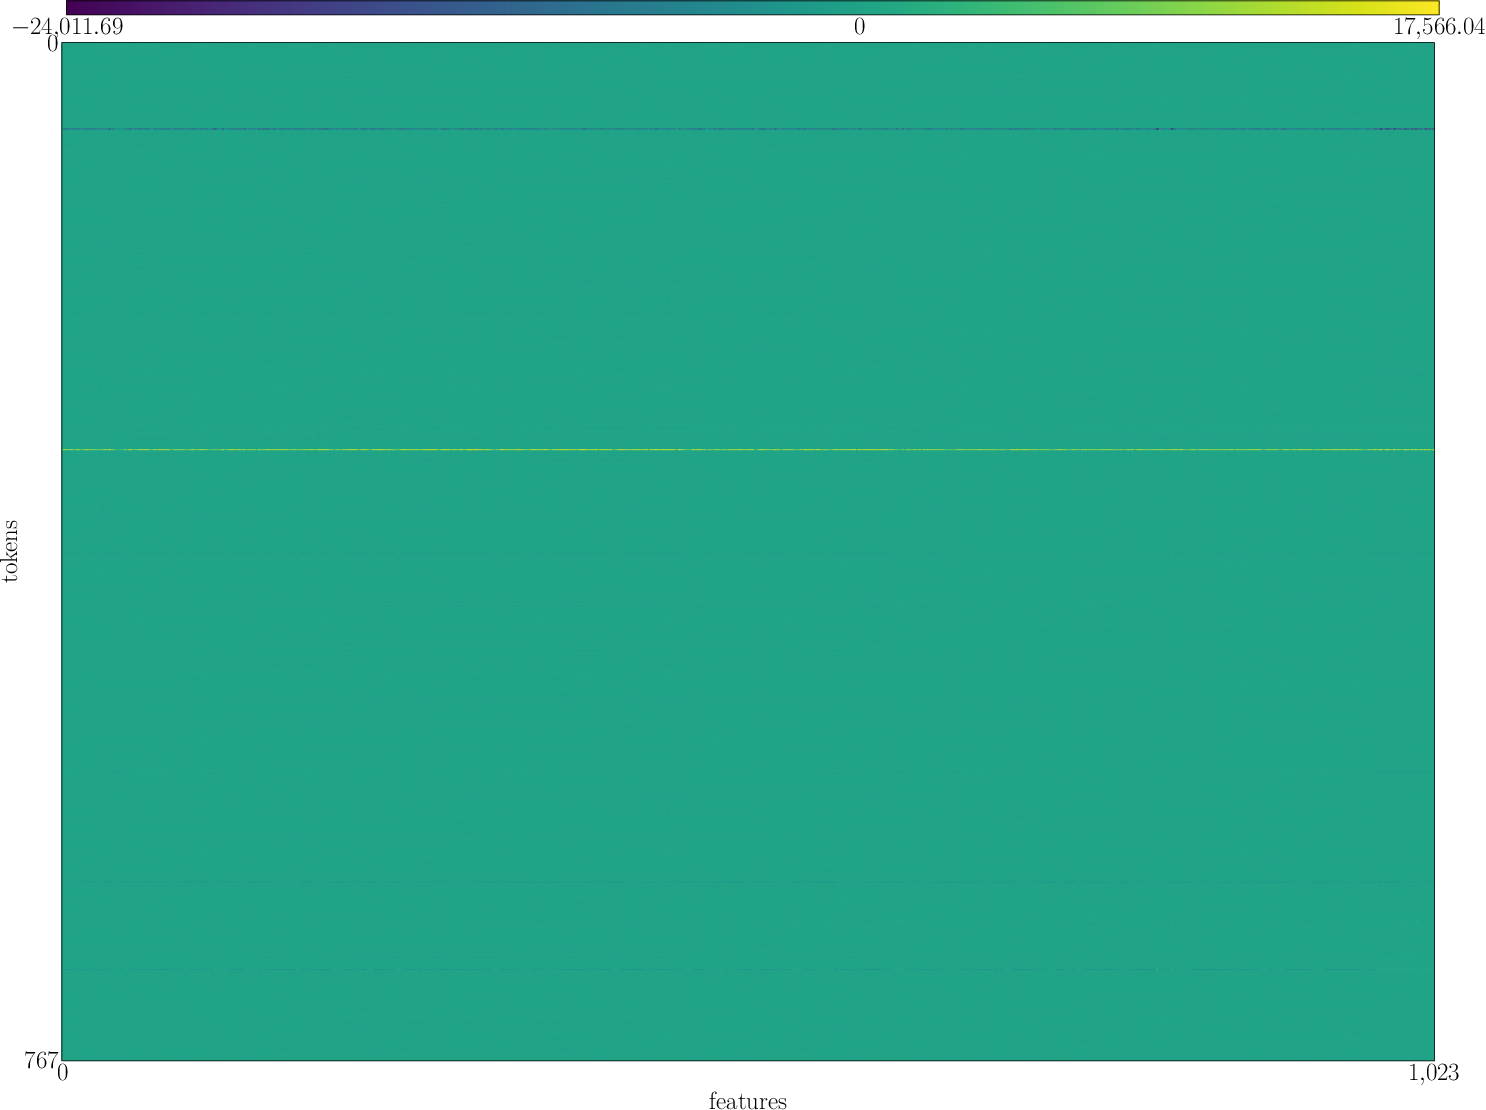
\includegraphics[width=\textwidth]{../res/sp16.png}
\end{figure}

\begin{figure}
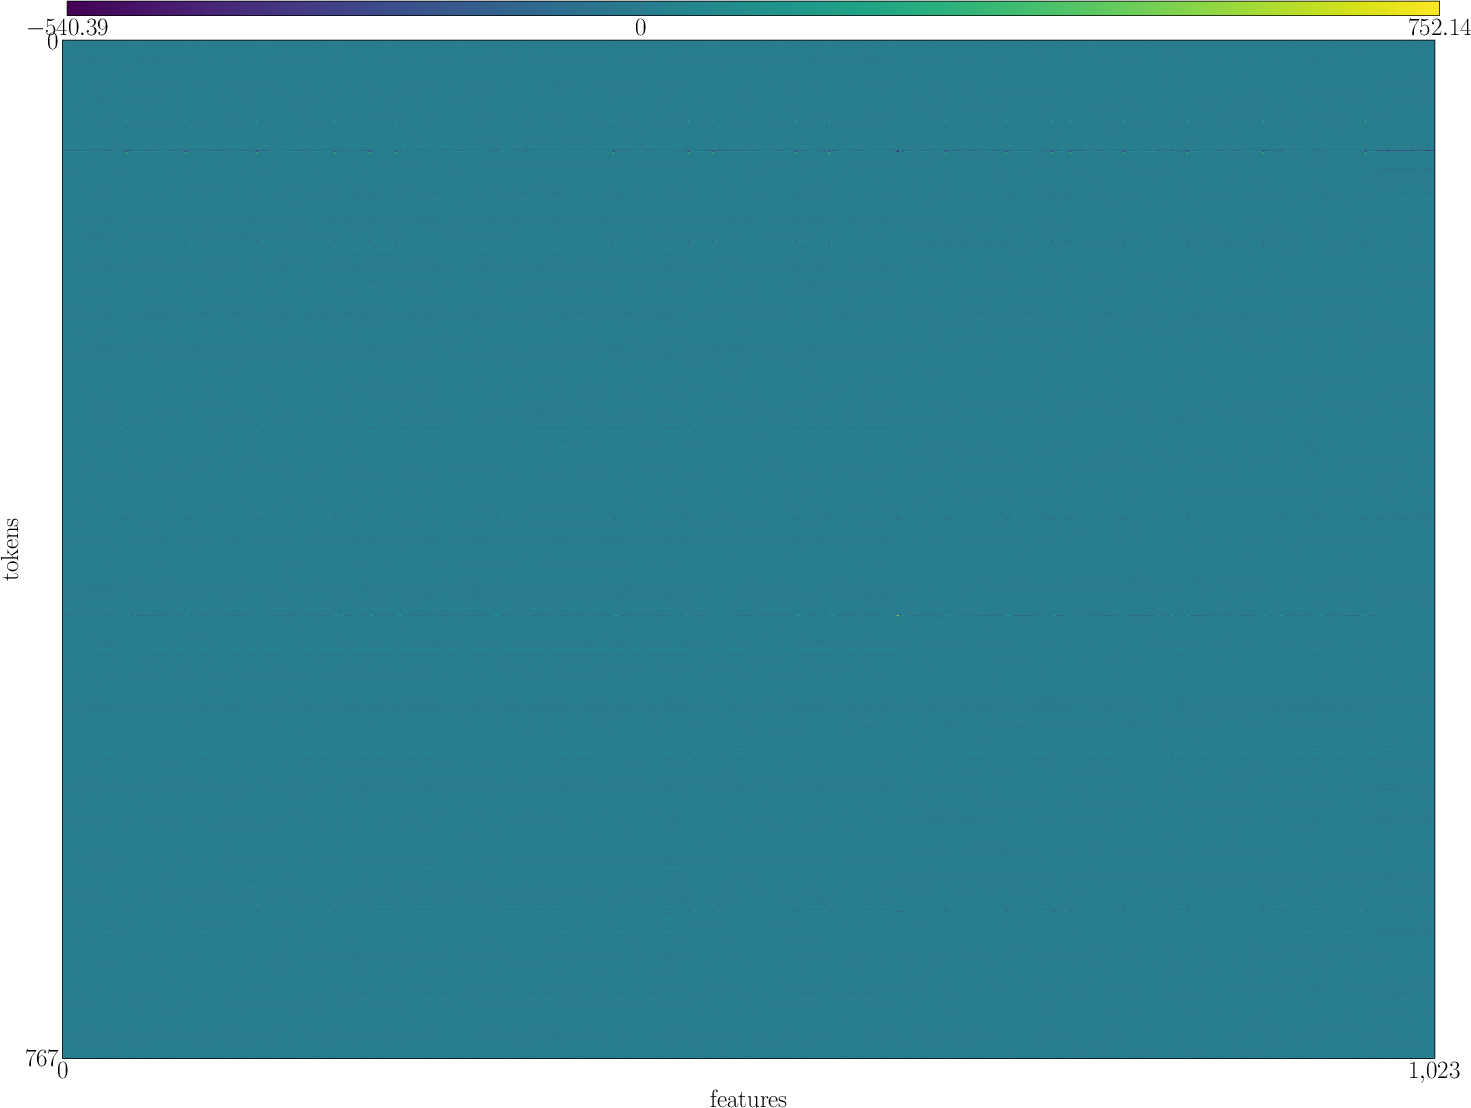
\includegraphics[width=\textwidth]{../res/mup16.png}
\end{figure}

\begin{table}[h!]
\Centering
\begin{tabular}{cccccccc}
\toprule
& Parametrization & mean & std & min & max & kurt & mmr\\
\midrule
\multirow{3}{*}{$\zeta=1$} & SP & \\
& \mup &\\
& \mup (threshold) &\\
\cmidrule{1-8}
\multirow{3}{*}{$\zeta=2$} & SP & \\
& \mup &\\
& \mup (threshold) &\\
\bottomrule
\end{tabular}
\caption{Distribution}
\end{table}

\begin{table}[h!]
\centering
\begin{tabular}{cccccccc}
\toprule
$\zeta$ & Parametrization & mean & std & min & max & kurt & mmr\\
\midrule
\multirow{3}{*}{$\zeta=1$} & SP & 0.06 & 3.64 & -25.10 & 23.77 & 4.14 & 6.91 \\
& \mup & 0 & 5.21 & -33.52 & 32.89 & 6.26 & 8.09 \\
& \mup (threshold) & -0.26 & 3.49 & -23.11 & 17.73 & 1.96 & 5.20 \\
\cmidrule{1-8}
\multirow{3}{*}{$\zeta=2$} & SP & -0.03 & 10.79 & -121.72 & 81.85 & 20.35 & 13.33 \\
& \mup & -0.14 & 6.45 & -81.05 & 71.61 & 11.72 & 9.12 \\
& \mup (threshold) & -0.03 & 4.80 & -29.48 & 50.60 & 11.03 & 9.79 \\
\cmidrule{1-8}
\multirow{3}{*}{$\zeta=4$} & SP & 0.02 & 30.75 & -661.47 & 357.34 & 75.95 & 30.40 \\
& \mup & -0.38 & 12.08 & -214.18 & 231.90 & 25.58 & 14.36 \\
& \mup (threshold) & 0.01 & 3.17 & -53.16 & 25.17 & 22.18 & 12.59 \\
\cmidrule{1-8}
\multirow{3}{*}{$\zeta=8$} & SP & -0.85 & 121.24 & -1974.84 & 3968.10 & 171.88 & 62.00 \\
& \mup & 0.15 & 11.78 & -184.89 & 568.77 & 102.74 & 30.43 \\
& \mup (threshold) & 0 & 3.34 & -58.35 & 87.03 & 82.16 & 24.09 \\
\cmidrule{1-8}
\multirow{3}{*}{$\zeta=16$} & SP & -3.30 & 489.38 & -24011.69 & 17566.04 & 442.83 & 136.87 \\
& \mup & 0.11 & 10.56 & -540.39 & 752.14 & 185.82 & 30.64 \\
& \mup (threshold) & -0.04 & 2.87 & -99.39 & 118.88 & 107.13 & 21.90 \\
\bottomrule
\end{tabular}
\caption{Distribution}
\end{table}

\subsection{Qualitative}

\section{Conclusion}
Indication/indicates

\printbibliography

\end{document}
